\chapter{取り扱うデータの条件}
科学的に事象を取り扱うための本書で扱うデータの条件は以下の通りである。
これらが無いならば、本書で扱える範囲を超えている。統計学者を専攻した科学者に相談した方が良い\footnote{最初から相談した方が良い}。

\begin{itemize}
    \item 再現性 同じような条件であれば、同じような現象が生じるということである。
    \item 計測誤差  計測により生じた誤差(測定誤差)は揺らぎ(集団内での差)に比べて十分に小さい
    \item 無作為抽出 なるべく偏りなく母集団からデータを取得する%母集団の特徴を捉えるためのデータの収集方法
    \item 実験デザイン バイアスを小さくなるように計画を行う。
    \item 予測 データを集めると、データとモデルの予測に関して相違点が明らかになり、モデルの改訂が必要になる。この改訂に終わりはない。
\end{itemize}

%みたいものを見るための計測方法がランダムサンプリングである。

\begin{SMbox}{何を学ばなければならないか}
    \cite{box1976science}から引用しておく。
    \begin{quote}
        We may ask of Fisher \\
        Was he an applied statistician? \\
        Was he a mathematical statistician?  \\
        Was he a data analyst? \\
        Was he a designer of investigations?\\
        It is surely because he was all of these that he was much more than the sum of the parts. He provides an example we can seek to follow. 
    \end{quote}
    %Fisherみたくなるのは難しいので、実験デザインと
\end{SMbox}

\section{実験デザイン}
わたしが扱える範囲ではないので、他書を読んだ方が良い。
今後まとめたい。
\begin{SMbox}{あとでまとめたいTODO}

    'Pseudoreplication' problem‐接着したコドラートは何が悪いのか
 \url{http://www.mus-nh.city.osaka.jp/iso/argo/nl02/nl02-21-32.html}
\end{SMbox}

\section{無作為抽出されていない事による過誤}
対象を無作為に抽出できていない標本から、統計量を計算し、モデルの母数を推定したとする。
このモデルでは、本来設定した母集団に関する予測には誤りが多くなる。
例えば、17歳の日本人男性の身長を母集団に指定したのに、17歳のバスケ部部員の身長を計測する。
その標本を元に、モデルの母数を推定し、母集団に関する推測を行う。
すると、その予測は母集団に関して十分なものではなくなる。
例えば、平均が大きくなりすぎたり、平均よりも小さな人の割合が予測と異なることが生じる。
%その標本を元に、想定していた母集団に関しての推測を行おうとする。
%そうしたとき、その予測は母集団に関して十分なものではなくなる。

やってはいけないとは言い切れないが、偏った集団を計測してしまった場合、
その解釈に一工夫が必要になる。


\subsection{Questionable Research Practice(QRP)}
以下ではやってはいけないことを紹介する。
国立研究開発法人 日本医療研究開発機構が出版している研究公正に関するヒヤリ・ハット集の
「7 研究データの信頼性、再現性等 」に詳しくまとめられている\footnote{\url{https://www.amed.go.jp/content/000064531.pdf}}。
% http://bunkei.ila.titech.ac.jp/sotsuronexcellence/class18_furui_kairi.pdf
\subsection{HARKing}
仮説が有無によらず、なんらかのデータを解析したあとに、その解析結果をもとに新たな仮説を構築する。さらに、あたかも元からその新たな仮説を検証することを目的とし研究をおこなったかのように偽り報告をおこなうこと。
このことを仮説ハッキング($HARKing$(Hypothesizing After the Results are Known))といい、研究不正である\footnote{
    HARKingは、再現性の問題という意見もある。
    \url{https://twitter.com/ykamit/status/1077716200845500416} 。母集団を無作為抽出していないことで、再現できないことが増えると考えられる。
}
\footnote{
    多重検定により、$p$値が低く推測されることが問題であるというものもある\cite{池田_功毅2016,中村_大輝2021sp20016}。部分的には同意できるが、私は十分理解できなかった。
}\footnote{
    Twitterでのアンケートでは、多くの人がHARkingをうまく理解できてないというTwitterでのアンケートもある。
    \url{https://twitter.com/biomedcircus/status/1088957697368690689}
}\footnote{
    探索的なデータ解析においては、帰無仮説の後付けが許されるという主張もある。この意見には同意できない。母集団について拡大解釈をすることは許されない。探索的データ解析により得られるのは、母集団かつ$p<\alpha$という集団が見つかったということのみ主張できる。
    これを元に、母集団に関する性質を言及してしまうのはおかしい。
    %母集団についての推測をしたと主張はできない。
}\footnote{
    HARKingについては、\cite{kerr1998harking}に詳しくまとめられている
}。

%https://twitter.com/Hiroshi12337131/status/1613560913889742849
% https://twitter.com/ykamit/status/1615162295986028546
% https://twitter.com/ykamit/status/1090791485312720896



\begin{SMbox}{HARKing}
    \begin{rightbubbles}{bubblegreen}{Yuki Kamitani}{./image/Twitter_logo_PNG/2021_Twitter_logo_blue.png}
        %{./section/image/Twitter_logo_EPS/2021_Twitter_logo_blue.eps}
    データを操作してp値をいじる行為を不正と認識している人は多いが、HARKingが不正と思っている人は非常に少ない。私の周辺分野のシニア研究者で理解している人はほぼ皆無(問題を指摘すると一笑に付される)。研究の実践と論文フォーマットの齟齬やフェアプレー精神の問題(?)と理解している人がいた
        \begin{flushright} 
            \small	\url{https://twitter.com/ykamit/status/1077715969827528705}
        \end{flushright}    
    \end{rightbubbles}
    
    HARkingを理解するのは、難しい。無作為抽出したデータから、データを調べた後に、母集団を構成しているのだから、無作為抽出できていると考えてしまいがちになる。
\end{SMbox}
 


\begin{SMbox}{学術分野によってことなるHARKingの認識}
    \begin{rightbubbles}{bubblegreen}{Takefumi Nakazawa}{./image/Twitter_logo_PNG/2021_Twitter_logo_blue.png}
        生態学では、データを取ってから研究の筋書き(イントロ)を考える事がある。研究の動機が対象への興味だったり、結果が予想と違う事が多かったりするからだろう。研究発表には新規性が必要なので、どうやって大きな新規性を謳うかのか、どういうイントロを構成するか、特に学生さんは悩むだろう。
        \begin{flushright} 
            \small	\url{https://twitter.com/Take_Nakazawa/status/1635760385436557312}
            \end{flushright}    
        \end{rightbubbles}

    \begin{rightbubbles}{bubblegreen}{Takefumi Nakazawa}{./image/Twitter_logo_PNG/2021_Twitter_logo_blue.png}
        新規性を謳うには、自分の材料や技術に捉われず、他の多くの研究事例の中で、自分の研究をできるだけ一般化する必要がある。攻めれば大風呂敷と言われ、守れば新規性が弱いと言われ、勉強不測のために新規性がないと言われることもある。この辺の「スキル」が上手な人は早く論文を書ける。
        \begin{flushright} 
            \small	\url{https://twitter.com/Take_Nakazawa/status/1635762588788326400}
            \end{flushright}    
        \end{rightbubbles}

        \begin{rightbubbles}{bubblegreen}{Takefumi Nakazawa}{./image/Twitter_logo_PNG/2021_Twitter_logo_blue.png}
            研究の材料と技術は研究室で提供され、体系的に習得しやすいが、筋書きを作る技術には、他の研究に関する知識に加えて、ある種のセンスが必要なのではないかと思う。知識は学べば得られるが、新規性を謳うには既存の知識を統合した上で、欠けている大きな穴を見つけなければいけないからだ。
            \begin{flushright} 
            \small	\url{https://twitter.com/Take_Nakazawa/status/1635764423599198208}
            \end{flushright}    
        \end{rightbubbles}

        \begin{rightbubbles}{bubblegreen}{Takefumi Nakazawa}{./image/Twitter_logo_PNG/2021_Twitter_logo_blue.png}
            生態学会で沢山のポスター発表を見て、こんなデータでこんな筋書きを作るのかと感じることが多々ある。きっと当初はそんな筋書きはなかったのだろう。始める前より面白い筋書きになって、寧ろ面白いと感じたかもしれない。データを取るだけではなく、これが生態学なのかって勉強した人もいるかも。
            \begin{flushright} 
            \small	\url{https://twitter.com/Take_Nakazawa/status/1635765545932042242}
            \end{flushright}    
        \end{rightbubbles}

        \begin{rightbubbles}{bubblegreen}{Takefumi Nakazawa}{./image/Twitter_logo_PNG/2021_Twitter_logo_blue.png}
            でも、本心で言えば、みんながみんな大風呂敷を広げて生態学の偉大な理論を見つけたかのように新規性を高らかに謳っている学会は、少し距離を置いてみてみると、異様な学会に見えたりもする。外部の人にとっては、何が重要な研究テーマ間の花、生態学は何を目指しているのか、わからないのではないか。
            \begin{flushright} 
            \small	\url{https://twitter.com/Take_Nakazawa/status/1635766641157087233}
            \end{flushright}    
        \end{rightbubbles}

        \begin{rightbubbles}{bubblegreen}{Takefumi Nakazawa}{./image/Twitter_logo_PNG/2021_Twitter_logo_blue.png}
            自然界は複雑で多様だから、そんなことは仕方がないし、それがむしろ面白いとは思う。時々見られる大風呂敷に感動することもある。でも、新規性の呪縛に捉われて、見ている現象や系の面白さが台無しになっているような発表もあったりして、心苦しく思うこともある。
            \begin{flushright} 
            \small	\url{https://twitter.com/Take_Nakazawa/status/1635768265611022336}
            \end{flushright}    
        \end{rightbubbles}
        \begin{rightbubbles}{bubblegreen}{Takefumi Nakazawa}{./image/Twitter_logo_PNG/2021_Twitter_logo_blue.png}
            研究発表の場だから、発表者は聴衆のために一般化された筋書きを用意しているだけかもしれない。センスのある筋書きはそれはそれで面白いけど、私が一番面白いと感じるのは、他人のために無理やりに一般化された筋書きではなく、本人が面白いと思って取ったデータをその思いのまま伝えた発表なのである
            \begin{flushright} 
            \small	\url{https://twitter.com/Take_Nakazawa/status/1635769045046919169}
            \end{flushright}    
        \end{rightbubbles}

        \begin{rightbubbles}{bubblegreen}{Ohkubo Yusaku}{./image/Twitter_logo_PNG/2021_Twitter_logo_blue.png}
            (ガチのフィールド研究室だったので「データからの筋書き」が生態学を駆動する大きな力であることは認めた上で、)幅広い学術領域でHARKingの問題が指摘されてる以上もう少し現状のプラクティスを見直すか、「データからの筋書き」を擁護する真面目な理屈を考える必要があるように思える。
            \begin{flushright} 
            \small	\url{https://twitter.com/Ohkubo2021/status/1637804153039917059}
            \end{flushright}    
        \end{rightbubbles}

        \begin{rightbubbles}{bubblegreen}{Takefumi Nakazawa}{./image/Twitter_logo_PNG/2021_Twitter_logo_blue.png}
            \url{https://journals.plos.org/plosone/article?id=10.1371/journal.pone.0200303}
            \begin{flushright} 
            \small	\url{https://twitter.com/Take_Nakazawa/status/1637832643567050754}
            \end{flushright}    
        \end{rightbubbles}
        
ある学術分野ではHARKingが行われている。「やってはいけないのになぜやってるんですか?」ときかれても困る。やってるのである。


\begin{rightbubbles}{bubblegreen}{Ken McAlinn}{./image/Twitter_logo_PNG/2021_Twitter_logo_blue.png}
    これは(広義の)研究不正だと思うんだけど、そういう認識がないんだろう。それ自体は仕方ないんだけど、悪いインセンティブが働きすぎで是正はかなり難しいように思う。
    引用\url{https://twitter.com/Take_Nakazawa/status/1635760385436557312}
    \begin{flushright} 
    \small	\url{https://twitter.com/kenmcalinn/status/1637816619605827584}
    \end{flushright}    
\end{rightbubbles}
\begin{rightbubbles}{bubblegreen}{ballman}{./image/Twitter_logo_PNG/2021_Twitter_logo_blue.png}
    これ書かれてる先生自身はその問題を認識さてるというのは置いといて、自分の友人でも生態学やってる人いますが統制された実験がそもそも可能かというところもあるので、分野的には探索探索で割り切ったらええんちゃうかなとは思います
    \begin{flushright} 
    \small	\url{https://twitter.com/katsuymd/status/1637819533355548672}
    \end{flushright}    
\end{rightbubbles}
\begin{rightbubbles}{bubblegreen}{Ken McAlinn}{./image/Twitter_logo_PNG/2021_Twitter_logo_blue.png}
    あまり研究不正として認識はしてないと思うんですよね。まぁ探索なら探索でいいんですけどね。
    \begin{flushright} 
    \small	\url{https://twitter.com/kenmcalinn/status/1637822015175262208}
    \end{flushright}    
\end{rightbubbles}

HARKingは研究不正。

\end{SMbox}

HARKingを意図せず生させてしまう状況をいくつか紹介する。
\subsubsection{後付けの母集団かつ$p<\alpha$を満たす集団}
母集団Aを設定し、標本を抽出したものを標本aとする。標本aのデータはさまざまな要素から構成されているとする。例えば、ある会社に所属する人の、身長や年収、税金の支払い履歴、ローン残高、労働部署、高校時代の部活などであるとする。
この標本から、何らかの属性$A'$に当てはまるデータbを抽出したとする。
データbについて特定の統計モデルとの乖離するかを調べ、乖離していることをが判明したとする(乖離を定量的に調べる方法はなんでもいいが、$p<\alpha$だったと考えても良い)。
この結果から、属性$A'$に関わると考えられる母集団A'を再構成する。
そこから、母集団$A'$を特定のモデルで予測できないと結論づけることはできない。

まず、今集めた標本$a$は、母集団$A$から集めたものであり、母集団$A'$から集めたものではない。
よって、母集団$A'$から無作為抽出できていない。
また、標本aを無作為抽出したときに付随して得た、母集団$A'$の一部の偏った集団のデータである。
以上から、母集団$A'$に関する無作為抽出とはいえない。
図\ref{fig:conceptual_diagram_HARKing}には、概念図を示しておいた。

\subsubsection{後付けの母集団かつ$p<\alpha$を満たす集団}
$p<\alpha$であるという標本がデータから発見されたので、標本の特性を持つと思われる母集団を後付けし、その母集団から無作為抽出を行なったことにし、ある統計モデルとデータが乖離していたと言うストーリーを作ったとする。
%統計モデルが棄却されたというストーリーを作ったとする。
言い換えれば、後付けの母集団ならば、$p<\alpha$であるという論理を立てたとする。
実際には、後付けの母集団でありかつ$p<\alpha$という集団から作為抽出しているので\footnote{この場合でも無作為抽出できていると誤解してしまうが、後付けの母集団から無作為抽出できていない!}、本来の母集団については何もわからない。言い換えれば、母集団に関する拡大解釈が行われたことで、母集団に関しては何もわからないのに、推測を行なったと主張している\footnote{実際調査した母集団は母集団かつ$p<0.05$に対して、報告した母集団デカすぎんだろ...}。
母集団の特徴を知るには、無作為抽出を行い、推測を行う必要がある。

\begin{figure}
    \begin{center}
        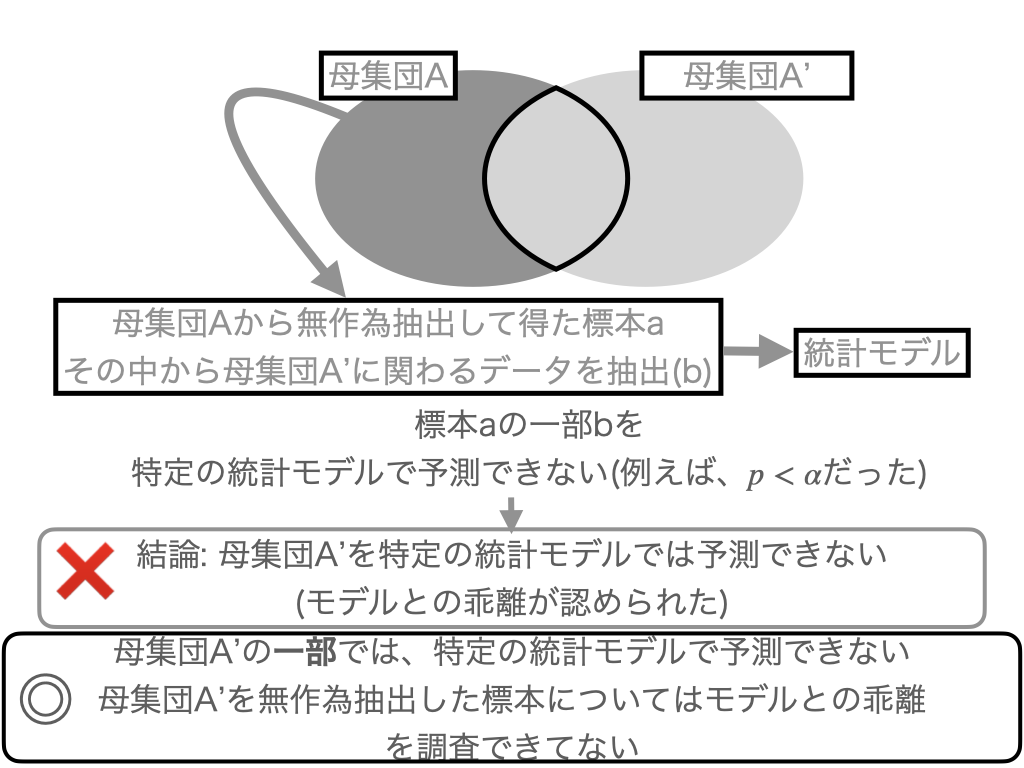
\includegraphics[bb=0 0 1024 768,width=15cm]{./image/01_/conceptual_diagram/conceptual_diagram.005.png}
        \caption{仮説ハッキングの概念図}
        \label{fig:conceptual_diagram_HARKing}
    \end{center}
\end{figure}
    

\subsubsection{仮説検証型にしなければいけない}
論文として投稿するときには、データから仮説を生成し、その仮説を検証したというように体裁をととのえるように要求されることが多々ある。

\begin{SMbox}{仮説検証型/仮説探索型}

\begin{rightbubbles}{bubblegreen}{
Satoshi Tanaka (@sato51643335)}{./image/Twitter_logo_PNG/2021_Twitter_logo_blue.png}
   論点が盛りだくさんでこの問題に詳しくないと理解しづらいかもしれません。検証的研究におけるHARKingは不正ですが、探索的研究では問題ではないので、誤解が起こらないと良いのですが。
    \begin{flushright} 
    \small	\url{https://twitter.com/sato51643335/status/1645911659213643776}
    \end{flushright}    
\end{rightbubbles}

仮説検証型または仮説探索型だとしても、計画し、実行したことそして、得られたデータを改竄/隠蔽なく報告することが必要である。

\end{SMbox}



\subsection{$p<\alpha$になったら無作為抽出を終える}
$p$値がある値を下回ったときに、実験を終了するという操作を行なったとする。
統計モデルの予測と一致するように、母集団を選択したことになる。
この場合、無作為抽出した集団により、設定した母集団に関する性質を調べるという研究目的を達成できない。
「母集団かつ設定したモデルにおいて$p<\alpha$である」集団に関する調査を行なっていることになる。

調査を終えて、この標本についてモデルを使った予測ができないと主張できない。
この不正な操作をアステリスクシーキングという。


\subsection{標本平均がxxになったときに抽出を終える}
標本に対して計算できる平均値や分散が理想の(考えているモデル)と一致するまで無作為抽出を繰り返すまたは、一致したときに無作為抽出を終えると、無作為抽出したとは言いきれない。


\begin{SMbox}{計測したデータを報告しない}
    \begin{quote}
        日本製鉄は18日、東日本製鉄所君津地区(千葉県君津市)から有害物質が流出していた問題で、過去の水質測定データに不適切な扱いがあったと発表した。排出基準を超える有害物質が検出されたにもかかわらず、千葉県などに報告していない例があった。有害物質が基準を上回った際、再度測定して基準内に収まる結果を記録していたことも明らかにした。
        \ \ \\ \url{https://www.nikkei.com/article/DGXZQOUC186070Y2A810C2000000/}
    \end{quote}

    アンモニア化合物の漏洩が発生し、着色水の構外への流出が確認され、排水溝から取水したサンプルから、環境規制値を超えるシアンが検出される   \footnote{東日本製鉄所君津地区における着色水の構外への流出について \url{https://www.nipponsteel.com/common/secure/news/20220624_100.pdf}}。
    その後、シアン除去設備の能力増強などが行われる\footnote{\url{https://www.nipponsteel.com/common/secure/news/20220706_100.pdf}}。
    さらに、精査していくと、測定データについて不適切な取り扱いがあったことが判明した\footnote{\url{https://www.nipponsteel.com/common/secure/news/20220818_200.pdf}}。
    ここで、1日のうちに複数回の計測データが存在していたこと、関係機関へ報告していた数値より高い計測データが存在していたことが判明した。

    計測データが、予想や基準値よりも大きかったまたは小さかったから、データを削除してはいけない。
    計測手順を決定し、そして計測したデータは、全て報告しなければならない。

    データが恣意的に削除されているかどうかを判定することは非常に難しい。
    この例でも、データを持たない外部の人間が、不適切な報告が行われていることを判定できなかった。
    基準値を超えたデータについても記録が残っていたので、報告が適切に行われていないことが明らかになった。


    データがなければ、どのような行動を行うだろうか。
    例えば、保存されたサンプルを再度計測することになる。
    そのサンプルがなければ、なぜ基準値を超えた値が検出されたのかが徹底的にせいさされることになる。例えば、計測装置の利用手順のミスなどが検証される。
    ここで異常がなければ、通常のサンプリングが行われ、基準値を超えるデータが取得される頻度が、これまでよりも高いかを調べることになると考えられる。
    データがなければ、検証のコストが増えてしまうと考えられる。

    
    %川が赤くなっているという報告が上がったこともあり、調査が行われたようである\footnote{\url{https://news.yahoo.co.jp/articles/ea20d54623642b848960d93404aad6eba3ffae4a}}

\end{SMbox}



\section{Garbage in, garbage out}

ある集団の統計的性質をモデルを使って調べたい。
特定のモデルにおいて発生頻度が著しく低い集団については、そのモデルで出現頻度に関して十分な予測ができない。
言い換えれば、モデルにおいてメジャーな集団における性質を調べるためには、モデルにおいて発生頻度の低い集団を省くことで、メジャーな集団の性質を理解しやすくなる。
そこで、データの中からいくつかを取り除くことが必要になる。


ゴミデータを統計処理したならば、ゴミのような推論しか得られない。言い換えれば、意味のある結果を返しにくくなったり、解釈が難しくなることがある。
このことをGarbage in, garbage outと呼ぶ。



特定の統計量を予想していた値に近づけるためにデータを取り除ってはいけない。
我々の行いたいことは、注目したい現象の統計的特徴を調べることである。

成功した実験結果と失敗した実験結果とで計測した数値が似ているにていたとする。この場合、すべてを混ぜて解析をおこなうと、統計量が過度に小さく推定される。
反対に、似た数値ではない場合、統計量は過度に大きく推定される\footnote{どちらかといえば、解析担当者が、なんとなくサンプルサイズは大きいほうがいいという気分があり、すべてを同一視して解析をしたいという気分になりがち。}。
%本章で指摘したデータの取り方を守っていないならば、そのデータを用いて統計処理を行ったとしても、一般的な事柄を推測・予想することは難しくなる。


\if 0
注意しなくてはならないことは、一般的な事柄に関する予測や推測を目的にしていないならば、本章で指摘したデータの取り方をしていないことがあり得る。
例えば、無作為抽出することができない実験はあり得る。
そこで得られたデータに価値が十分ある\footnote{良い例を探すべき。}。%\url{http://www.mus-nh.city.osaka.jp/iso/argo/nl02/nl02-21-32.html}}。
\fi

\subsection{実験手順を守っていないデータ}
実験手順を守っていないデータを何ら断りも入れずに、手順を守ったデータと同一視し、解析すると、統計量を過大・過小評価しやすくなる。

\subsection{再現できなかったデータ}
ある手順に沿って実験を行ったとしても常に同一の結果が得られないことがある。
例えば、次のようなことが考えられる。
\begin{itemize}
    \item 動物に休眠を誘発する薬剤を投与したにもかかわらず、休眠しなかった
    \item ある遺伝子が発現するように手順を踏んだにもかかわらず発現しなかった
\end{itemize}
いずれもその後、ある量を計測し、それを解析するという手順だとする。
同一視できない現象のデータを混ぜて解析することは辞めておいたほうがいい。

解析対象とした結果が生じた数と実験回数も報告の対象になる。報告しなければ、データの隠蔽と判断されかねない。


\subsection{外れ値}
外れ値とは、手順通りに行ったサンプルにおいて、想定していた計測値から著しく離れた値をとったサンプルのこである。
想定がなければサンプル内において注目する集団を恣意的に決定し、それ以外を外れ値として処理することになる。

どのような基準を用いてサンプルを外したのかや実験手順を元に行われた全サンプルの数も、報告の対象になる。




\section{みにくいアヒルの子の定理}
恣意的に特徴量を選ばなければ、ある共通点をもつ2つの物に関して、類似した特徴の個数と類似しない特徴の個数は、同数になることを示唆する。
\if 0
適当に取ってきた特徴によって二つの物を区別しようとすると、区別できることが多々あり、特徴をあげれるだけあげてその中から1つ選んだとすれば、$50\%$くらいは二つのことがらを区別できる特徴である。
次のような実験を計画する。まず、二つの事柄に関してあげれるだけ特徴をあげ、一つずつ特徴を取って調べて、異なっているとみなせるかを判断する。異なるといえそうなものが見つかったら、実験計画を練って、再び実験を行い、その特徴に関する仮説がすでにあったかのようにして報告を行う。
いつかは分類可能な特徴を得られるはずなので、やめておいた方が良い。研究目的を立てて、特徴となるデータを取っていくことが通常の研究方法である。

恣意的に選ばなくても、異なると判断できる特徴が見つけることができることを示唆している。
また、我々が分類を行うさいに、恣意的に特徴を選んで物を区別していることを示唆している。
\fi
%https://atmarkit.itmedia.co.jp/ait/articles/2007/30/news024.html
%https://ibisforest.org/index.php?%E9%86%9C%E3%81%84%E3%82%A2%E3%83%92%E3%83%AB%E3%81%AE%E5%AD%90%E3%81%AE%E5%AE%9A%E7%90%86
%https://www.nri.com/-/media/Corporate/jp/Files/PDF/knowledge/publication/kinyu_itf/2016/06/itf_201606_10.pdf?la=ja-JP&hash=8E8C1FF018D272D3AE358EABEB0D1B82370AEE9C
% https://ibisforest.org/index.php?%E9%86%9C%E3%81%84%E3%82%A2%E3%83%92%E3%83%AB%E3%81%AE%E5%AD%90%E3%81%AE%E5%AE%9A%E7%90%86

\if 0
\section{教示あり学習におけるノーフリーランチ定理}
この定理の誤解した解釈なので書かない方がいい
汎化誤差が平均的に同等になるという定理である。
あらゆる問題に対して性能の良いモデルは理論上存在しない。また、あるモデルが他のモデルよりも良い性能を示すのは、現在解こうとしている問題に特化している場合に限る。

既存モデルが新しいデータに対して適合的でなことは多々あり、そのデータを組み込み、提案した提案モデルの方がデータに適合することを示唆している。

\fi


\if 0
自分の言葉に書き換えよう
\begin{quote}
    もしアルゴリズムが、ある特定領域の問題において優れた性能を発揮しているのなら、それ以外の残り全ての問題群においては性能が低下する代償を支払う必要がある
    \url{https://atmarkit.itmedia.co.jp/ait/articles/2007/17/news020.html}    
\end{quote}
\fi 


\if 0
\section{統計学の理解に関するバイアス}
生物学の現場では、黒魔術的な統計学を使っていることがある。言い過ぎになるかもしれないが、黒魔術を習得し、論文を書いていかなければ、生物学者にはなれない。
彼らは、黒魔術を後輩のために教え続け、黒魔術を習得したもののみが生物学者として認められていく。
査読システムが悪いんじゃぁ
%このように黒魔術を行なったもののみが生き残れる環境が作り出されていく。

\fi

